\documentclass[11pt,a4paper]{article}

\usepackage{datetime}
\usepackage{graphicx}
\usepackage{enumitem}
\usepackage{amsmath}
\usepackage{subcaption}

\usepackage{hyperref}

\hypersetup{
    colorlinks=true,
    linkcolor=blue,
    filecolor=magenta,      
    urlcolor=cyan,
}

\title{Chapter 6 Lab Work: Synchronization}
\newdate{date}{05}{06}{2020}
\date{\displaydate{date}}
\author{Nguyen Ngoc Lam - 20162316}

\begin{document}
\pagenumbering{gobble}
\maketitle
\newpage
\pagenumbering{arabic}
\tableofcontents
\newpage

\section{Launch this program several times. What do you notice? Explain it!}
There are some times when the program print out the wrong answer (expected 3000 every time, got less than 3000 at some instances)
\begin{figure}[h!]
	\centering
  	\begin{subfigure}[b]{0.4\linewidth}
  		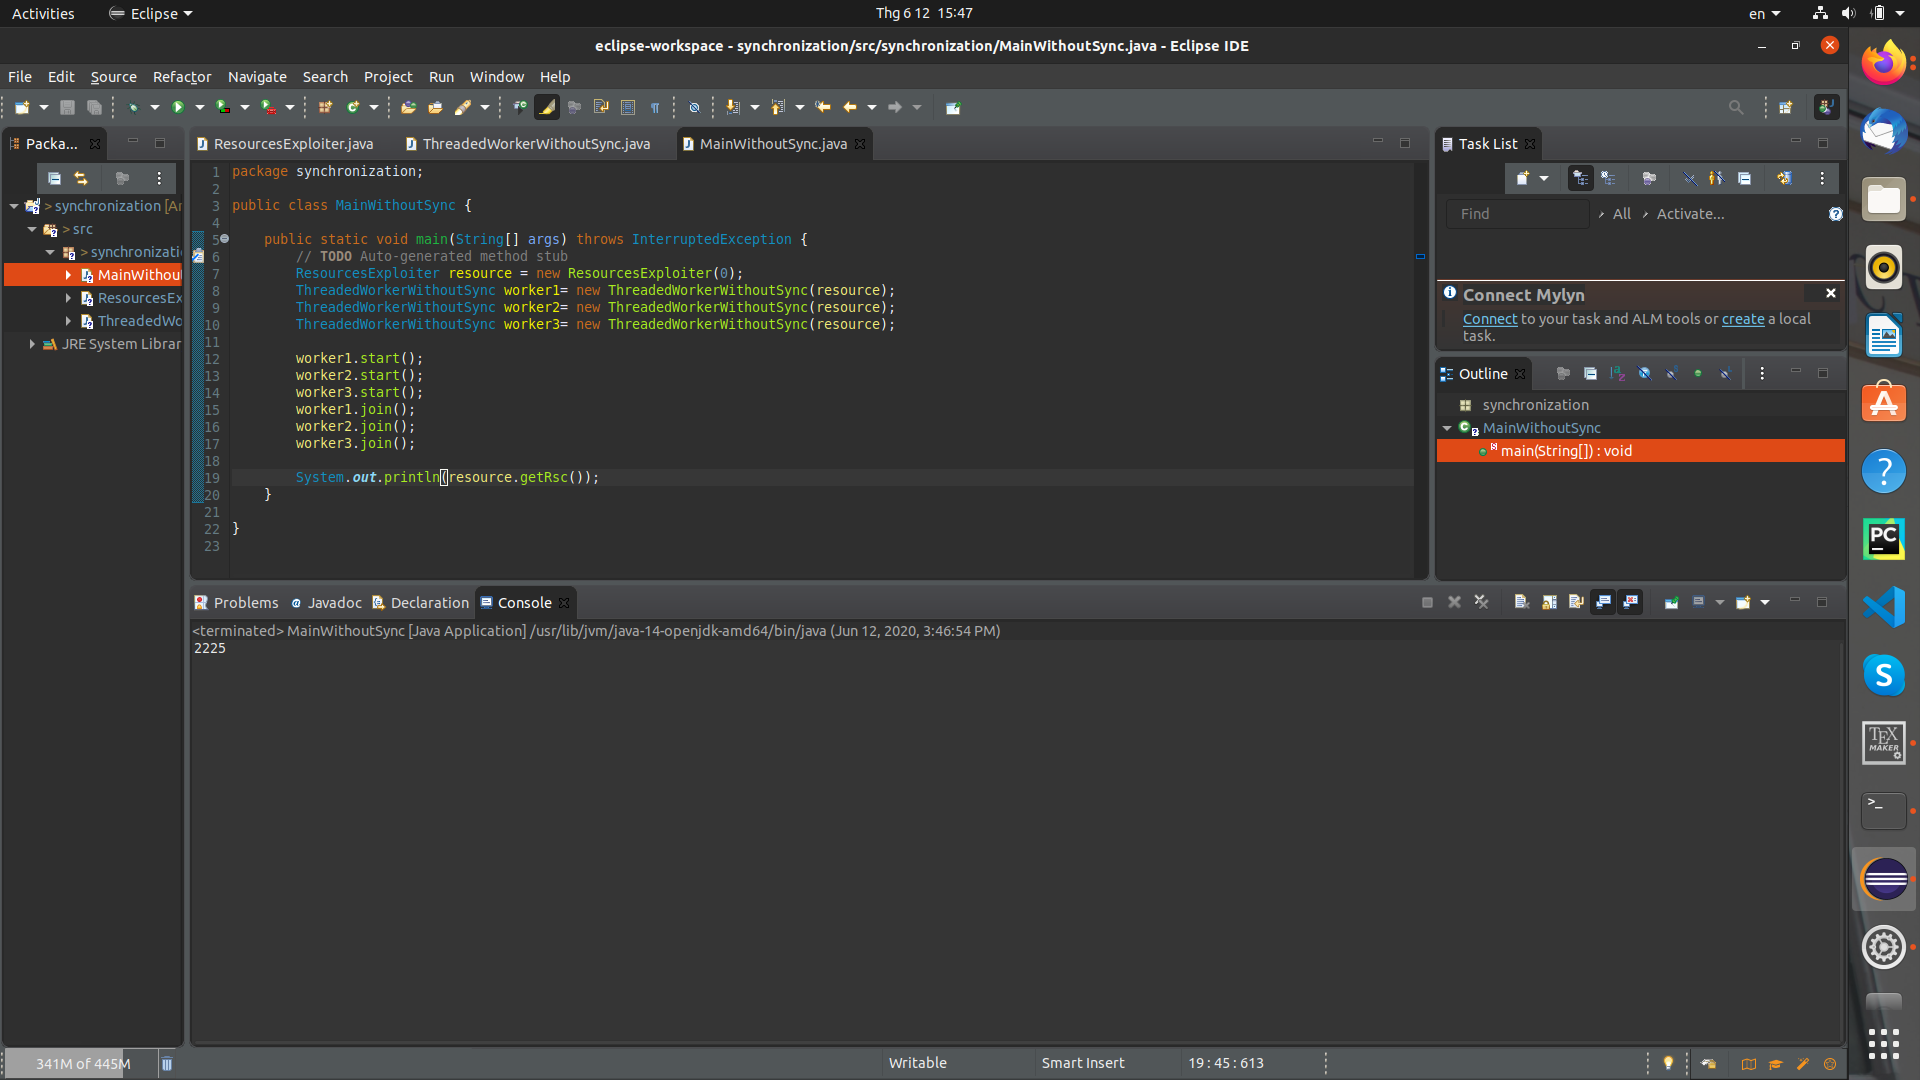
\includegraphics[width=\linewidth]{less-3000.png}
    	\caption{Unexpected result}
  	\end{subfigure}
  	\begin{subfigure}[b]{0.4\linewidth}
    	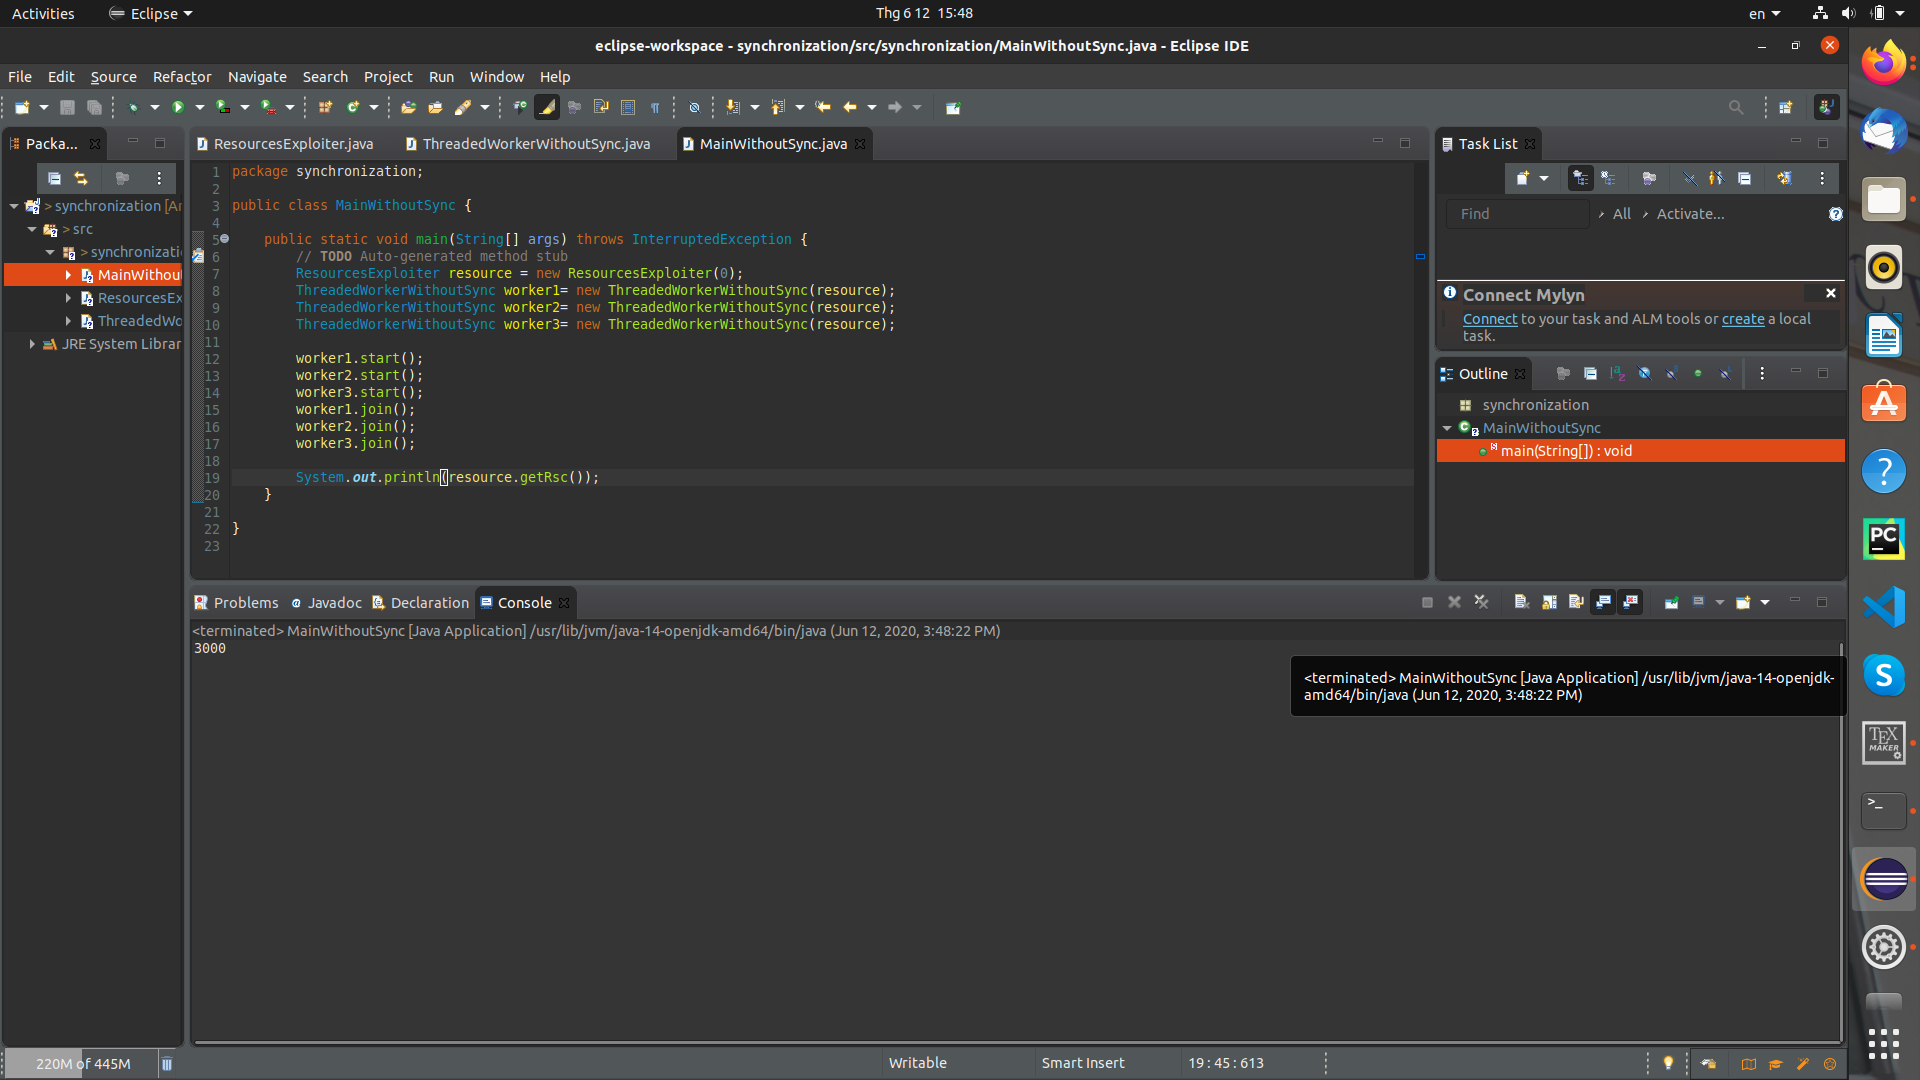
\includegraphics[width=\linewidth]{exact-3000.png}
    	\caption{The right result}
  	\end{subfigure}
  	\caption{Two types of result}
  	\label{fig:wosync}
\end{figure}
\\\textbf{Explanation:} Since there is not synchronization between each worker, sometimes two workers will try to access the resource at the same time. Each one, get the old value and add 1 to that and return the resource. Because of that, there are "less" addition happened and led to smaller result.
\section{Differences after synchronization. Explain}
The result is now consistently 3000 due to applying synchronization that makes workers access the resource in an "orderly" fashion.
\section{Differences after using lock. Explain}
The result is now consistently 3000 due to applying lock mechanism that makes only one worker can access the resource at one time.
\section{Complete this file above (in the part YOUR-CODE-HERE) with a loop to increase the variable shared by 1 for 5 seconds.}

\section{Try to increase the value of threads and the value of the constant NUM\_TRANS after each execution time until you obtain the different results between Balance and INIT\_BALANCE $+$ credits $-$ debits. Explain why do you get this difference.}
\begin{figure}[h!]
	\centering
  	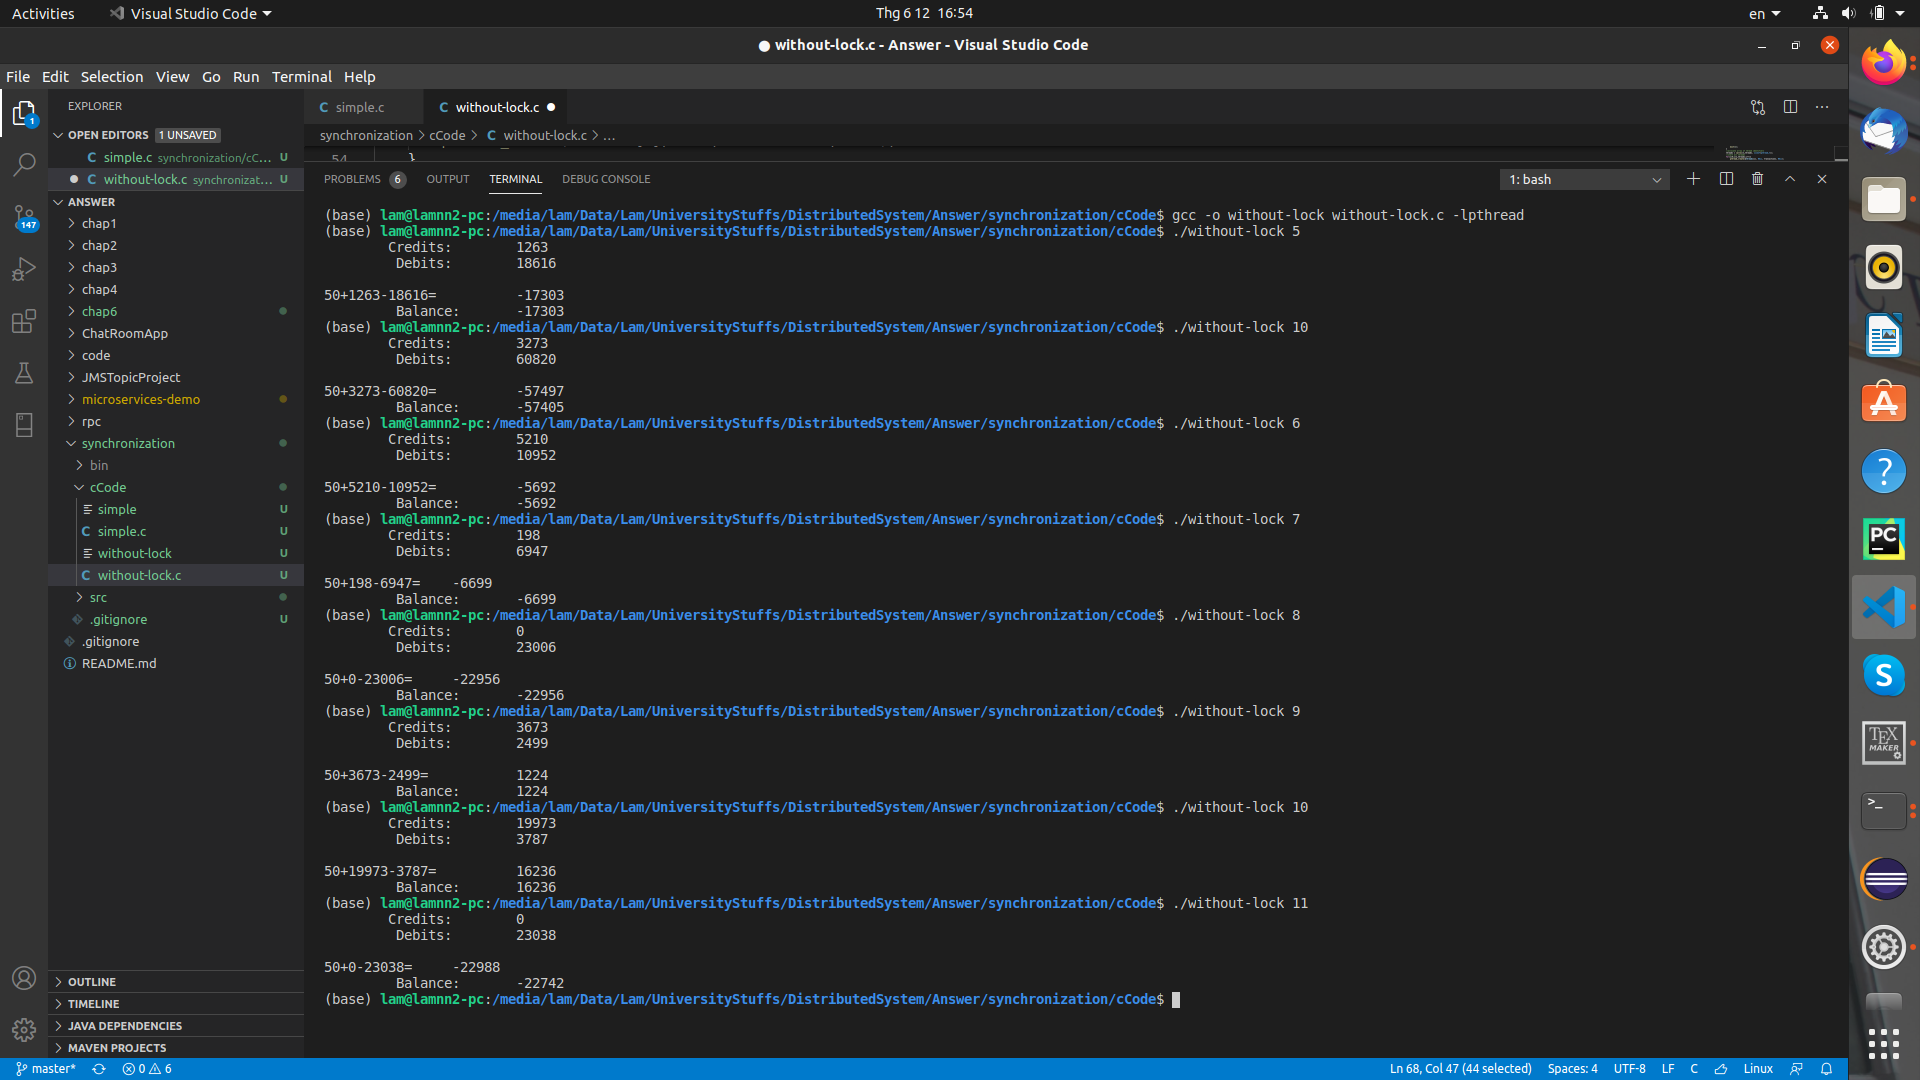
\includegraphics[width=\linewidth]{without-lock.png}
  	\caption{Result when there is not any lock}
  	\label{fig:wolock}
\end{figure}
Since every threads can access freely to the resource, when calculate the balance and there are more than one thread try to calculate that, it will not return the desired result (the whole operations of N thread involved) instead it updates the value according to the last to complete it operation. The higher the number of threads, the bigger chance of this to happened. The save option would be to make variable credits and debits exclusively used of each other and each thread only performs a credit or debit but not both.

\section{Try to build and run this program. Launch it repeatedly until you see the difference between Shared and Expect values. Analyze the source code to understand the problem that leads to this difference.}
\begin{figure}[h!]
	\centering
  	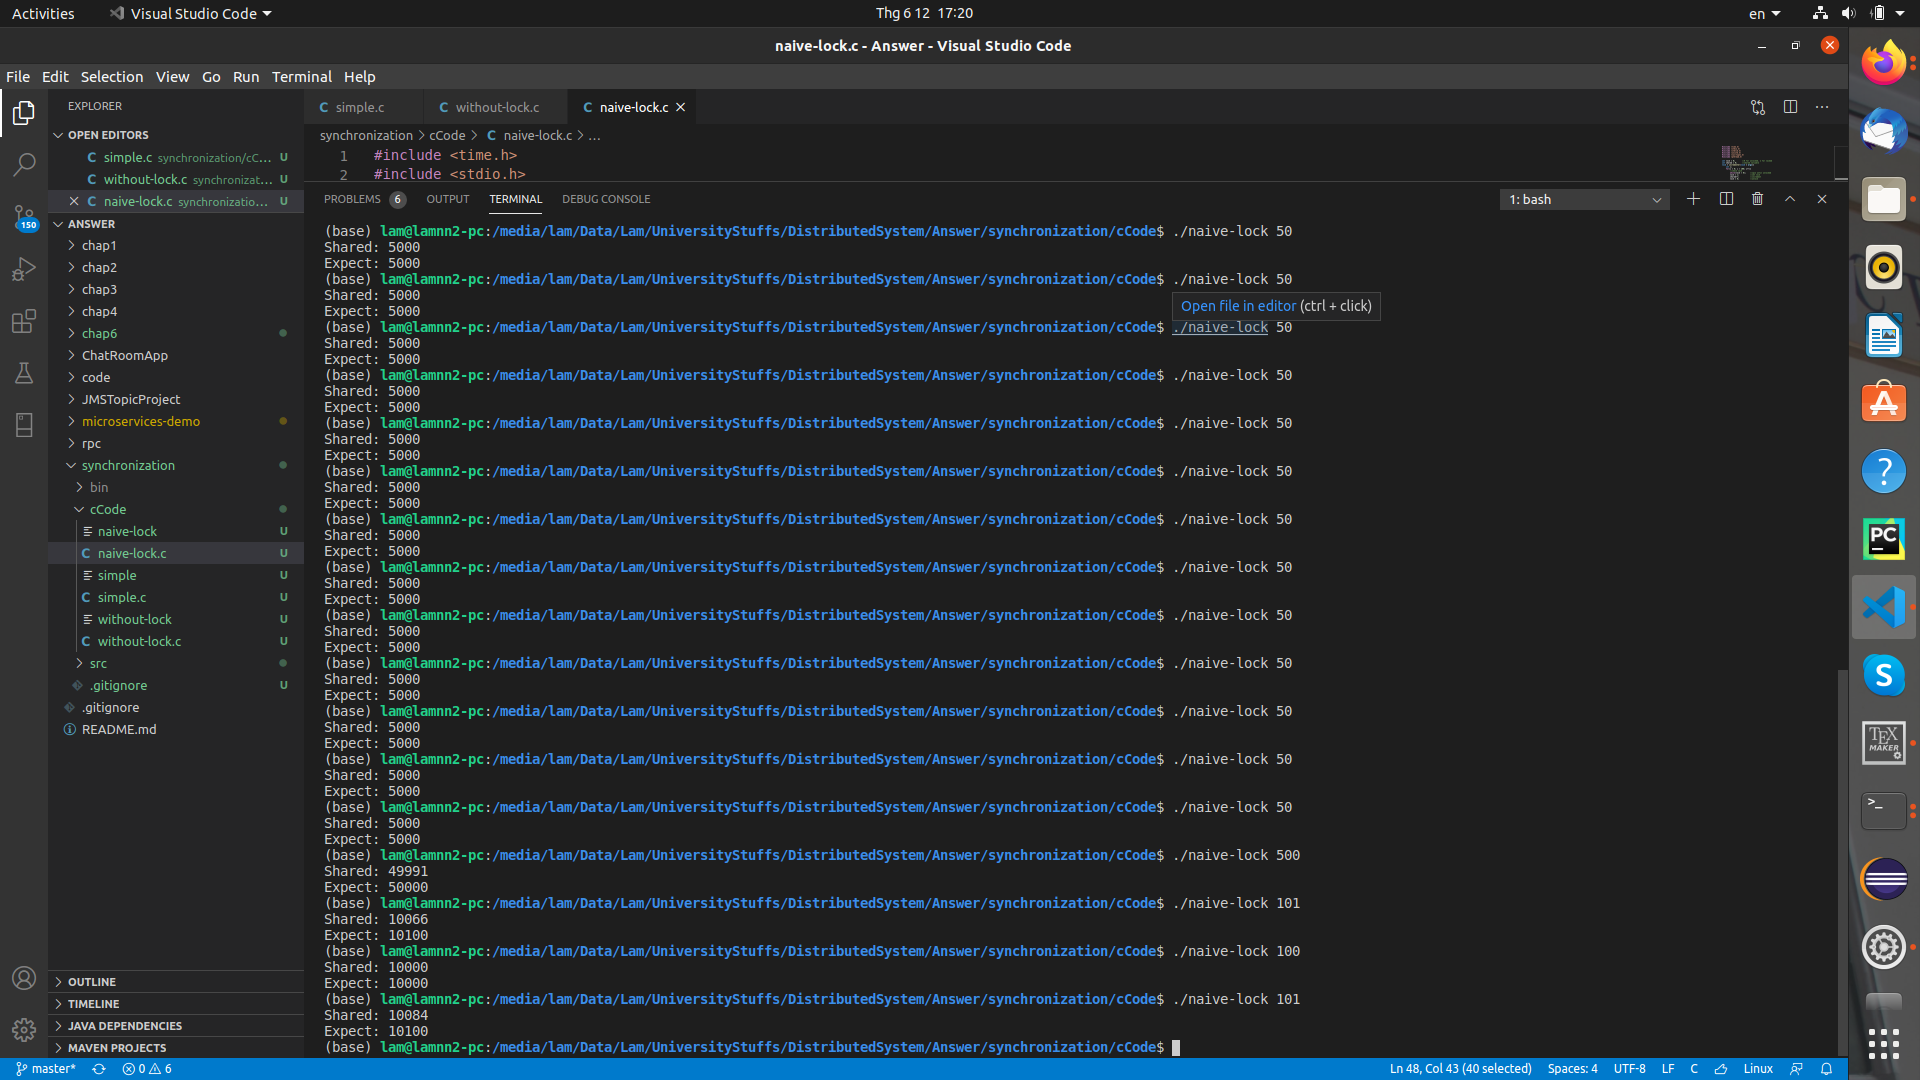
\includegraphics[width=\linewidth]{naive-lock.png}
  	\caption{Result when using naive lock}
  	\label{fig:naivelock}
\end{figure}
Since naive lock can only work for when the number of thread is smaller than 100 (as declared in the increment function), if the number of threads is larger than 100, it will immediately have a problem.

\section{What is the improvement after using mutex lock}
When use mutex lock, I saw that the number of error reduced dramatically. The error rate is nearly zero (out of all the time I run the program it return the different answer once). 

\section{Compare the run times of the two strategies to prove that Fine Locking is faster and much faster on larger load sets}
On 10000 threads, Coarse Locking runs in about 3 seconds. Meanwhile, Fine Locking runs in about 1.5 seconds.

\section{Run this program and what do you get as output? Explain what the deadlock is}
The program will forever runs and it never give the output.\\
Deadlock: deadlock is a state in which each member of a group is waiting for another member, including itself, to take action, such as sending a message or more commonly releasing a lock. In this particular problem, fun\_1 gets the lock of resource a first while fun\_2 gets the lock of resource b. 2 processes need both lock to work, but since neither can acquire the pair of locks so they will forever wait each other.
\end{document}